\documentclass[a4paper, 14pt]{extarticle}
\usepackage[utf8]{inputenc}
\usepackage[paper=a4paper, top=1cm, right=1cm, bottom=1.5cm, left=2cm]{geometry}
\usepackage{setspace}
\onehalfspacing

\usepackage{graphicx}
\graphicspath{{plots/}, {images/}}

\parindent=1.25cm

\usepackage{titlesec}

\titleformat{\section}
    {\normalsize\bfseries}
    {\thesection}
    {1em}{}

\titleformat{\subsection}
    {\normalsize\bfseries}
    {\thesubsection}
    {1em}{}

% Настройка вертикальных и горизонтальных отступов
\titlespacing*{\chapter}{0pt}{-30pt}{8pt}
\titlespacing*{\section}{\parindent}{*4}{*4}
\titlespacing*{\subsection}{\parindent}{*4}{*4}

\usepackage[square, numbers, sort&compress]{natbib}
\makeatletter
\bibliographystyle{unsrt}
\renewcommand{\@biblabel}[1]{#1.} 
\makeatother


\newcommand{\maketitlepage}[6]{
    \begin{titlepage}
        \singlespacing
        \newpage
        \begin{center}
            Министерство образования и науки Российской Федерации \\
            Федеральное государственное бюджетное образовательное \\
            учреждение высшего профессионального образования \\
            <<Волгоградский государственный технический университет>> \\
            #1 \\
            Кафедра #2
        \end{center}


        \vspace{14em}

        \begin{center}
            \large Семестровая работа #6 по дисциплине
            \\ <<#3>>
        \end{center}

        \vspace{5em}

        \begin{flushright}
            \begin{minipage}{.35\textwidth}
                Выполнила:\\#4
                \vspace{1em}\\
                Проверил:\\#5
                \\
                \\ Оценка \underline{\ \ \ \ \ \ \ \ \ \ \ \ \ \ \ \ }
            \end{minipage}
        \end{flushright}

        \vspace{\fill}

        \begin{center}
            Волгоград, \the\year
        \end{center}

    \end{titlepage}
    \setcounter{page}{2}
}

\newcommand{\maketitlepagewithvariant}[7]{
    \begin{titlepage}
        \singlespacing
        \newpage

        \begin{center}
            Министерство образования и науки Российской Федерации \\
            Федеральное государственное бюджетное образовательное \\
            учреждение высшего профессионального образования \\
            <<Волгоградский государственный технический университет>> \\
            #1 \\
            Кафедра #2
        \end{center}


        \vspace{8em}

        \begin{center}
            \large Семестровая работа #6 по дисциплине
            \\ <<#3>>
        \end{center}

        \vspace{1em}
        \begin{center}
            Вариант №#7
        \end{center}
        \vspace{4em}

        \begin{flushright}
            \begin{minipage}{.35\textwidth}
                Выполнила:\\#4
                \vspace{1em}\\
                Проверил:\\#5
                \\
                \\ Оценка \underline{\ \ \ \ \ \ \ \ \ \ \ \ \ \ \ \ }
            \end{minipage}
        \end{flushright}

        \vspace{\fill}

        \begin{center}
            Волгоград, \the\year
        \end{center}

    \end{titlepage}
    \setcounter{page}{2}
}

\input{../../../../.preambles/10-russian}
\input{../../../../.preambles/20-math}
\input{../../../../.preambles/22-vectors}
\input{../../../../.preambles/30-physics}
\usepackage{mathrsfs}

\newcommand{\ds}{\displaystyle}
\newcommand{\inv}{\mathrm{inv}}
\renewcommand{\v}{\mathrm{v}}
\newcommand{\E}{\mathscr{E}}

\begin{document}
\maketitlepage{Факультет электроники и вычислительной техники}{физики}
{Электродинамика}{2}{}{студент группы Ф-369\\Чечеткин~И.~А.}{m}
{доцент Грецов~М.~В.}{m}

\newpage
% ------------------------------------------------------------------------------
\emph{698.} Определить закон движения частицы во взаимно перпендикулярных
однородных постоянных электрическом \( \vec{E} \) и магнитном \( \vec{B} \)
полях. Сделать это двумя способами:
\vspace*{-1em}
\begin{enumerate}\itemsep-.5em
    \item используя преобразование Лоренца и считая известным движение частицы в
    чисто электрическом или чисто магнитном поле;
    \item интегрируя следующие уравнения:
    \begin{equation}
        \der{p_i}{\tau} = eF^i, \quad
        m\der{u_i}{\tau} = \frac{e}{c}F_{ik}u_k.
        \label{eq:1_task}
    \end{equation}
\end{enumerate}

\vspace*{2em}
\emph{Решение:}
\begin{enumerate}
    \item Примем, что в системе \( S \) электрическое поле \( E \| y \), а
    магнитное \( B \| z \). Пусть в начальный момент частица находилась в начале
    координат \( x = y = z = 0 \) и имела импульс \( \vec{p}_0 \).
    
    Движение будет различным в зависимости от соотношений между величинами
    \( E \) и \( B \).
    
    Если \( E > B \), то, как следует из инвариантов поля \( \vec{E}\cdot\vec{B}
    = \inv = 0 \) и \( E^2 - B^2 = \inv > 0 \), существует такая система отсчета
    \( S' \), в которой отсутствует магнитное поле.
    
    Из преобразования Лоренца для магнитного поля \( \vec{B} \)
    следует, что система \( S' \) должна двигаться относительно \( S \)
    параллельно оси \( x \) со скоростью \( \v = cB/E \).
    
    \_\_\_\_\_\_\_\_\_\_\_\_\_\_\_\_\_\_\_\_\_\_\_\_\_\_\_\_\_\_\_\_\_\_\_\_\_\_
    \!\!\_\_\_\_\_\_\_\_\_\_\_\_\_\_\_\_\_\_\_\_\_\_\_\_\_\_\_\_\\
    \_\_\_\_\_\_\_\_\_\_\_\_\_\_\_\_\_\_\_\_\_\_\_\_\_\_\_\_\_\_\_\_\_\_\_\_\_\_
    \!\!\_\_\_\_\_\_\_\_\_\_\_\_\_\_\_\_\_\_\_\_\_\_\_\_\_\_\_\_\\
    \_\_\_\_\_\_\_\_\_\_\_\_\_\_\_\_\_\_\_\_\_\_\_\_\_\_\_\_\_\_\_\_\_\_\_\_\_\_
    \!\!\_\_\_\_\_\_\_\_\_\_\_\_\_\_\_\_\_\_\_\_\_\_\_\_\_\_\_\_\\
    \_\_\_\_\_\_\_\_\_\_\_\_\_\_\_\_\_\_\_\_\_\_\_\_\_\_\_\_\_\_\_\_\_\_\_\_\_\_
    \!\!\_\_\_\_\_\_\_\_\_\_\_\_\_\_\_\_\_\_\_\_\_\_\_\_\_\_\_\_\\
    \_\_\_\_\_\_\_\_\_\_\_\_\_\_\_\_\_\_\_\_\_\_\_\_\_\_\_\_\_\_\_\_\_\_\_\_\_\_
    \!\!\_\_\_\_\_\_\_\_\_\_\_\_\_\_\_\_\_\_\_\_\_\_\_\_\_\_\_\_\\
    \_\_\_\_\_\_\_\_\_\_\_\_\_\_\_\_\_\_\_\_\_\_\_\_\_\_\_\_\_\_\_\_\_\_\_\_\_\_
    \!\!\_\_\_\_\_\_\_\_\_\_\_\_\_\_\_\_\_\_\_\_\_\_\_\_\_\_\_\_\\
    \_\_\_\_\_\_\_\_\_\_\_\_\_\_\_\_\_\_\_\_\_\_\_\_\_\_\_\_\_\_\_\_\_\_\_\_\_\_
    \!\!\_\_\_\_\_\_\_\_\_\_\_\_\_\_\_\_\_\_\_\_\_\_\_\_\_\_\_\_\\
    \_\_\_\_\_\_\_\_\_\_\_\_\_\_\_\_\_\_\_\_\_\_\_\_\_\_\_\_\_\_\_\_\_\_\_\_\_\_
    \!\!\_\_\_\_\_\_\_\_\_\_\_\_\_\_\_\_\_\_\_\_\_\_\_\_\_\_\_\_\\
    \_\_\_\_\_\_\_\_\_\_\_\_\_\_\_\_\_\_\_\_\_\_\_\_\_\_\_\_\_\_\_\_\_\_\_\_\_\_
    \!\!\_\_\_\_\_\_\_\_\_\_\_\_\_\_\_\_\_\_\_\_\_\_\_\_\_\_\_\_\\
    \_\_\_\_\_\_\_\_\_\_\_\_\_\_\_\_\_\_\_\_\_\_\_\_\_\_\_\_\_\_\_\_\_\_\_\_\_\_
    \!\!\_\_\_\_\_\_\_\_\_\_\_\_\_\_\_\_\_\_\_\_\_\_\_\_\_\_\_\_\\
    \_\_\_\_\_\_\_\_\_\_\_\_\_\_\_\_\_\_\_\_\_\_\_\_\_\_\_\_\_\_\_\_\_\_\_\_\_\_
    \!\!\_\_\_\_\_\_\_\_\_\_\_\_\_\_\_\_\_\_\_\_\_\_\_\_\_\_\_\_\\
    \_\_\_\_\_\_\_\_\_\_\_\_\_\_\_\_\_\_\_\_\_\_\_\_\_\_\_\_\_\_\_\_\_\_\_\_\_\_
    \!\!\_\_\_\_\_\_\_\_\_\_\_\_\_\_\_\_\_\_\_\_\_\_\_\_\_\_\_\_\\
    \_\_\_\_\_\_\_\_\_\_\_\_\_\_\_\_\_\_\_\_\_\_\_\_\_\_\_\_\_\_\_\_\_\_\_\_\_\_
    \!\!\_\_\_\_\_\_\_\_\_\_\_\_\_\_\_\_\_\_\_\_\_\_\_\_\_\_\_\_\\
    \_\_\_\_\_\_\_\_\_\_\_\_\_\_\_\_\_\_\_\_\_\_\_\_\_\_\_\_\_\_\_\_\_\_\_\_\_\_
    \!\!\_\_\_\_\_\_\_\_\_\_\_\_\_\_\_\_\_\_\_\_\_\_\_\_\_\_\_\_\\
    \_\_\_\_\_\_\_\_\_\_\_\_\_\_\_\_\_\_\_\_\_\_\_\_\_\_\_\_\_\_\_\_\_\_\_\_\_\_
    \!\!\_\_\_\_\_\_\_\_\_\_\_\_\_\_\_\_\_\_\_\_\_\_\_\_\_\_\_\_\\
    \_\_\_\_\_\_\_\_\_\_\_\_\_\_\_\_\_\_\_\_\_\_\_\_\_\_\_\_\_\_\_\_\_\_\_\_\_\_
    \!\!\_\_\_\_\_\_\_\_\_\_\_\_\_\_\_\_\_\_\_\_\_\_\_\_\_\_\_\_\\
    \_\_\_\_\_\_\_\_\_\_\_\_\_\_\_\_\_\_\_\_\_\_\_\_\_\_\_\_\_\_\_\_\_\_\_\_\_\_
    \!\!\_\_\_\_\_\_\_\_\_\_\_\_\_\_\_\_\_\_\_\_\_\_\_\_\_\_\_\_\\
    \_\_\_\_\_\_\_\_\_\_\_\_\_\_\_\_\_\_\_\_\_\_\_\_\_\_\_\_\_\_\_\_\_\_\_\_\_\_
    \!\!\_\_\_\_\_\_\_\_\_\_\_\_\_\_\_\_\_\_\_\_\_\_\_\_\_\_\_\_\\
    \_\_\_\_\_\_\_\_\_\_\_\_\_\_\_\_\_\_\_\_\_\_\_\_\_\_\_\_\_\_\_\_\_\_\_\_\_\_
    \!\!\_\_\_\_\_\_\_\_\_\_\_\_\_\_\_\_\_\_\_\_\_\_\_\_\_\_\_\_\\
    \_\_\_\_\_\_\_\_\_\_\_\_\_\_\_\_\_\_\_\_\_\_\_\_\_\_\_\_\_\_\_\_\_\_\_\_\_\_
    \!\!\_\_\_\_\_\_\_\_\_\_\_\_\_\_\_\_\_\_\_\_\_\_\_\_\_\_\_\_\\
    \_\_\_\_\_\_\_\_\_\_\_\_\_\_\_\_\_\_\_\_\_\_\_\_\_\_\_\_\_\_\_\_\_\_\_\_\_\_
    \!\!\_\_\_\_\_\_\_\_\_\_\_\_\_\_\_\_\_\_\_\_\_\_\_\_\_\_\_\_\\
    \_\_\_\_\_\_\_\_\_\_\_\_\_\_\_\_\_\_\_\_\_\_\_\_\_\_\_\_\_\_\_\_\_\_\_\_\_\_
    \!\!\_\_\_\_\_\_\_\_\_\_\_\_\_\_\_\_\_\_\_\_\_\_\_\_\_\_\_\_\\
    \_\_\_\_\_\_\_\_\_\_\_\_\_\_\_\_\_\_\_\_\_\_\_\_\_\_\_\_\_\_\_\_\_\_\_\_\_\_
    \!\!\_\_\_\_\_\_\_\_\_\_\_\_\_\_\_\_\_\_\_\_\_\_\_\_\_\_\_\_\\
    \_\_\_\_\_\_\_\_\_\_\_\_\_\_\_\_\_\_\_\_\_\_\_\_\_\_\_\_\_\_\_\_\_\_\_\_\_\_
    \!\!\_\_\_\_\_\_\_\_\_\_\_\_\_\_\_\_\_\_\_\_\_\_\_\_\_\_\_\_\\
    \_\_\_\_\_\_\_\_\_\_\_\_\_\_\_\_\_\_\_\_\_\_\_\_\_\_\_\_\_\_\_\_\_\_\_\_\_\_
    \!\!\_\_\_\_\_\_\_\_\_\_\_\_\_\_\_\_\_\_\_\_\_\_\_\_\_\_\_\_\\
    \_\_\_\_\_\_\_\_\_\_\_\_\_\_\_\_\_\_\_\_\_\_\_\_\_\_\_\_\_\_\_\_\_\_\_\_\_\_
    \!\!\_\_\_\_\_\_\_\_\_\_\_\_\_\_\_\_\_\_\_\_\_\_\_\_\_\_\_\_\\
    \_\_\_\_\_\_\_\_\_\_\_\_\_\_\_\_\_\_\_\_\_\_\_\_\_\_\_\_\_\_\_\_\_\_\_\_\_\_
    \!\!\_\_\_\_\_\_\_\_\_\_\_\_\_\_\_\_\_\_\_\_\_\_\_\_\_\_\_\_\\
    \_\_\_\_\_\_\_\_\_\_\_\_\_\_\_\_\_\_\_\_\_\_\_\_\_\_\_\_\_\_\_\_\_\_\_\_\_\_
    \!\!\_\_\_\_\_\_\_\_\_\_\_\_\_\_\_\_\_\_\_\_\_\_\_\_\_\_\_\_\\
    \_\_\_\_\_\_\_\_\_\_\_\_\_\_\_\_\_\_\_\_\_\_\_\_\_\_\_\_\_\_\_\_\_\_\_\_\_\_
    \!\!\_\_\_\_\_\_\_\_\_\_\_\_\_\_\_\_\_\_\_\_\_\_\_\_\_\_\_\_\\
    \_\_\_\_\_\_\_\_\_\_\_\_\_\_\_\_\_\_\_\_\_\_\_\_\_\_\_\_\_\_\_\_\_\_\_\_\_\_
    \!\!\_\_\_\_\_\_\_\_\_\_\_\_\_\_\_\_\_\_\_\_\_\_\_\_\_\_\_\_\\
        
    \item Дифференциальные уравнения движения имеют вид:
    \[
        \dder{x}{\tau} = \frac{qB}{mc}\der{y}{\tau}, \quad
        \dder{y}{\tau} = \frac{qE}{mc}\der{(ct)}{\tau} - \frac{qB}{mc}
        \der{x}{\tau}, \quad \dder{z}{\tau} = 0, \quad
        \dder{(ct)}{\tau} = \frac{qE}{mc}\der{y}{\tau},
    \]
    где \( \tau \) -- собственное время частицы.
    
    Пусть в начальный момент частица находилась в начале координат
    \( x = y = z = 0 \) и имела импульс \( \vec{p}_0 \).
    
    Интегрируя эту систему со следующими начальными условиями (\( \tau = 0
    \)):
    \[
        x = y = z = ct = 0,\ \pder{x}{\tau} = \frac{p_{0x}}{m},\ \pder{y}{\tau}
        = \frac{p_{0y}}{m},\ \pder{z}{\tau} = \frac{p_{0z}}{m},\ с\pder{t}{\tau}
        = \frac{\E_0}{mc},
    \]
    где \( \E_0 = \sqrt{c^2|\vec{p}_0|^2 + m^2c^4} \), найдем
    
    \_\_\_\_\_\_\_\_\_\_\_\_\_\_\_\_\_\_\_\_\_\_\_\_\_\_\_\_\_\_\_\_\_\_\_\_\_\_
    \!\!\_\_\_\_\_\_\_\_\_\_\_\_\_\_\_\_\_\_\_\_\_\_\_\_\_\_\_\_\\
    \_\_\_\_\_\_\_\_\_\_\_\_\_\_\_\_\_\_\_\_\_\_\_\_\_\_\_\_\_\_\_\_\_\_\_\_\_\_
    \!\!\_\_\_\_\_\_\_\_\_\_\_\_\_\_\_\_\_\_\_\_\_\_\_\_\_\_\_\_\\
    \_\_\_\_\_\_\_\_\_\_\_\_\_\_\_\_\_\_\_\_\_\_\_\_\_\_\_\_\_\_\_\_\_\_\_\_\_\_
    \!\!\_\_\_\_\_\_\_\_\_\_\_\_\_\_\_\_\_\_\_\_\_\_\_\_\_\_\_\_\\
    \_\_\_\_\_\_\_\_\_\_\_\_\_\_\_\_\_\_\_\_\_\_\_\_\_\_\_\_\_\_\_\_\_\_\_\_\_\_
    \!\!\_\_\_\_\_\_\_\_\_\_\_\_\_\_\_\_\_\_\_\_\_\_\_\_\_\_\_\_\\
    \_\_\_\_\_\_\_\_\_\_\_\_\_\_\_\_\_\_\_\_\_\_\_\_\_\_\_\_\_\_\_\_\_\_\_\_\_\_
    \!\!\_\_\_\_\_\_\_\_\_\_\_\_\_\_\_\_\_\_\_\_\_\_\_\_\_\_\_\_\\
    \_\_\_\_\_\_\_\_\_\_\_\_\_\_\_\_\_\_\_\_\_\_\_\_\_\_\_\_\_\_\_\_\_\_\_\_\_\_
    \!\!\_\_\_\_\_\_\_\_\_\_\_\_\_\_\_\_\_\_\_\_\_\_\_\_\_\_\_\_\\
    \_\_\_\_\_\_\_\_\_\_\_\_\_\_\_\_\_\_\_\_\_\_\_\_\_\_\_\_\_\_\_\_\_\_\_\_\_\_
    \!\!\_\_\_\_\_\_\_\_\_\_\_\_\_\_\_\_\_\_\_\_\_\_\_\_\_\_\_\_\\
    \_\_\_\_\_\_\_\_\_\_\_\_\_\_\_\_\_\_\_\_\_\_\_\_\_\_\_\_\_\_\_\_\_\_\_\_\_\_
    \!\!\_\_\_\_\_\_\_\_\_\_\_\_\_\_\_\_\_\_\_\_\_\_\_\_\_\_\_\_\\
    \_\_\_\_\_\_\_\_\_\_\_\_\_\_\_\_\_\_\_\_\_\_\_\_\_\_\_\_\_\_\_\_\_\_\_\_\_\_
    \!\!\_\_\_\_\_\_\_\_\_\_\_\_\_\_\_\_\_\_\_\_\_\_\_\_\_\_\_\_\\
    \_\_\_\_\_\_\_\_\_\_\_\_\_\_\_\_\_\_\_\_\_\_\_\_\_\_\_\_\_\_\_\_\_\_\_\_\_\_
    \!\!\_\_\_\_\_\_\_\_\_\_\_\_\_\_\_\_\_\_\_\_\_\_\_\_\_\_\_\_\\
    \_\_\_\_\_\_\_\_\_\_\_\_\_\_\_\_\_\_\_\_\_\_\_\_\_\_\_\_\_\_\_\_\_\_\_\_\_\_
    \!\!\_\_\_\_\_\_\_\_\_\_\_\_\_\_\_\_\_\_\_\_\_\_\_\_\_\_\_\_\\
    \_\_\_\_\_\_\_\_\_\_\_\_\_\_\_\_\_\_\_\_\_\_\_\_\_\_\_\_\_\_\_\_\_\_\_\_\_\_
    \!\!\_\_\_\_\_\_\_\_\_\_\_\_\_\_\_\_\_\_\_\_\_\_\_\_\_\_\_\_\\
    \_\_\_\_\_\_\_\_\_\_\_\_\_\_\_\_\_\_\_\_\_\_\_\_\_\_\_\_\_\_\_\_\_\_\_\_\_\_
    \!\!\_\_\_\_\_\_\_\_\_\_\_\_\_\_\_\_\_\_\_\_\_\_\_\_\_\_\_\_\\
    \_\_\_\_\_\_\_\_\_\_\_\_\_\_\_\_\_\_\_\_\_\_\_\_\_\_\_\_\_\_\_\_\_\_\_\_\_\_
    \!\!\_\_\_\_\_\_\_\_\_\_\_\_\_\_\_\_\_\_\_\_\_\_\_\_\_\_\_\_\\
    \_\_\_\_\_\_\_\_\_\_\_\_\_\_\_\_\_\_\_\_\_\_\_\_\_\_\_\_\_\_\_\_\_\_\_\_\_\_
    \!\!\_\_\_\_\_\_\_\_\_\_\_\_\_\_\_\_\_\_\_\_\_\_\_\_\_\_\_\_\\
    \_\_\_\_\_\_\_\_\_\_\_\_\_\_\_\_\_\_\_\_\_\_\_\_\_\_\_\_\_\_\_\_\_\_\_\_\_\_
    \!\!\_\_\_\_\_\_\_\_\_\_\_\_\_\_\_\_\_\_\_\_\_\_\_\_\_\_\_\_\\
    \_\_\_\_\_\_\_\_\_\_\_\_\_\_\_\_\_\_\_\_\_\_\_\_\_\_\_\_\_\_\_\_\_\_\_\_\_\_
    \!\!\_\_\_\_\_\_\_\_\_\_\_\_\_\_\_\_\_\_\_\_\_\_\_\_\_\_\_\_\\
    \_\_\_\_\_\_\_\_\_\_\_\_\_\_\_\_\_\_\_\_\_\_\_\_\_\_\_\_\_\_\_\_\_\_\_\_\_\_
    \!\!\_\_\_\_\_\_\_\_\_\_\_\_\_\_\_\_\_\_\_\_\_\_\_\_\_\_\_\_\\
    \_\_\_\_\_\_\_\_\_\_\_\_\_\_\_\_\_\_\_\_\_\_\_\_\_\_\_\_\_\_\_\_\_\_\_\_\_\_
    \!\!\_\_\_\_\_\_\_\_\_\_\_\_\_\_\_\_\_\_\_\_\_\_\_\_\_\_\_\_\\
    \_\_\_\_\_\_\_\_\_\_\_\_\_\_\_\_\_\_\_\_\_\_\_\_\_\_\_\_\_\_\_\_\_\_\_\_\_\_
    \!\!\_\_\_\_\_\_\_\_\_\_\_\_\_\_\_\_\_\_\_\_\_\_\_\_\_\_\_\_\\
    \_\_\_\_\_\_\_\_\_\_\_\_\_\_\_\_\_\_\_\_\_\_\_\_\_\_\_\_\_\_\_\_\_\_\_\_\_\_
    \!\!\_\_\_\_\_\_\_\_\_\_\_\_\_\_\_\_\_\_\_\_\_\_\_\_\_\_\_\_\\
    \_\_\_\_\_\_\_\_\_\_\_\_\_\_\_\_\_\_\_\_\_\_\_\_\_\_\_\_\_\_\_\_\_\_\_\_\_\_
    \!\!\_\_\_\_\_\_\_\_\_\_\_\_\_\_\_\_\_\_\_\_\_\_\_\_\_\_\_\_\\
    \_\_\_\_\_\_\_\_\_\_\_\_\_\_\_\_\_\_\_\_\_\_\_\_\_\_\_\_\_\_\_\_\_\_\_\_\_\_
    \!\!\_\_\_\_\_\_\_\_\_\_\_\_\_\_\_\_\_\_\_\_\_\_\_\_\_\_\_\_\\
    \_\_\_\_\_\_\_\_\_\_\_\_\_\_\_\_\_\_\_\_\_\_\_\_\_\_\_\_\_\_\_\_\_\_\_\_\_\_
    \!\!\_\_\_\_\_\_\_\_\_\_\_\_\_\_\_\_\_\_\_\_\_\_\_\_\_\_\_\_\\
    \_\_\_\_\_\_\_\_\_\_\_\_\_\_\_\_\_\_\_\_\_\_\_\_\_\_\_\_\_\_\_\_\_\_\_\_\_\_
    \!\!\_\_\_\_\_\_\_\_\_\_\_\_\_\_\_\_\_\_\_\_\_\_\_\_\_\_\_\_\\
    \_\_\_\_\_\_\_\_\_\_\_\_\_\_\_\_\_\_\_\_\_\_\_\_\_\_\_\_\_\_\_\_\_\_\_\_\_\_
    \!\!\_\_\_\_\_\_\_\_\_\_\_\_\_\_\_\_\_\_\_\_\_\_\_\_\_\_\_\_\\
    \_\_\_\_\_\_\_\_\_\_\_\_\_\_\_\_\_\_\_\_\_\_\_\_\_\_\_\_\_\_\_\_\_\_\_\_\_\_
    \!\!\_\_\_\_\_\_\_\_\_\_\_\_\_\_\_\_\_\_\_\_\_\_\_\_\_\_\_\_\\
    \_\_\_\_\_\_\_\_\_\_\_\_\_\_\_\_\_\_\_\_\_\_\_\_\_\_\_\_\_\_\_\_\_\_\_\_\_\_
    \!\!\_\_\_\_\_\_\_\_\_\_\_\_\_\_\_\_\_\_\_\_\_\_\_\_\_\_\_\_\\
    \_\_\_\_\_\_\_\_\_\_\_\_\_\_\_\_\_\_\_\_\_\_\_\_\_\_\_\_\_\_\_\_\_\_\_\_\_\_
    \!\!\_\_\_\_\_\_\_\_\_\_\_\_\_\_\_\_\_\_\_\_\_\_\_\_\_\_\_\_\\
    \_\_\_\_\_\_\_\_\_\_\_\_\_\_\_\_\_\_\_\_\_\_\_\_\_\_\_\_\_\_\_\_\_\_\_\_\_\_
    \!\!\_\_\_\_\_\_\_\_\_\_\_\_\_\_\_\_\_\_\_\_\_\_\_\_\_\_\_\_\\
    \_\_\_\_\_\_\_\_\_\_\_\_\_\_\_\_\_\_\_\_\_\_\_\_\_\_\_\_\_\_\_\_\_\_\_\_\_\_
    \!\!\_\_\_\_\_\_\_\_\_\_\_\_\_\_\_\_\_\_\_\_\_\_\_\_\_\_\_\_\\
    \_\_\_\_\_\_\_\_\_\_\_\_\_\_\_\_\_\_\_\_\_\_\_\_\_\_\_\_\_\_\_\_\_\_\_\_\_\_
    \!\!\_\_\_\_\_\_\_\_\_\_\_\_\_\_\_\_\_\_\_\_\_\_\_\_\_\_\_\_\\
    \_\_\_\_\_\_\_\_\_\_\_\_\_\_\_\_\_\_\_\_\_\_\_\_\_\_\_\_\_\_\_\_\_\_\_\_\_\_
    \!\!\_\_\_\_\_\_\_\_\_\_\_\_\_\_\_\_\_\_\_\_\_\_\_\_\_\_\_\_\\
    \_\_\_\_\_\_\_\_\_\_\_\_\_\_\_\_\_\_\_\_\_\_\_\_\_\_\_\_\_\_\_\_\_\_\_\_\_\_
    \!\!\_\_\_\_\_\_\_\_\_\_\_\_\_\_\_\_\_\_\_\_\_\_\_\_\_\_\_\_\\
    \_\_\_\_\_\_\_\_\_\_\_\_\_\_\_\_\_\_\_\_\_\_\_\_\_\_\_\_\_\_\_\_\_\_\_\_\_\_
    \!\!\_\_\_\_\_\_\_\_\_\_\_\_\_\_\_\_\_\_\_\_\_\_\_\_\_\_\_\_\\
    \_\_\_\_\_\_\_\_\_\_\_\_\_\_\_\_\_\_\_\_\_\_\_\_\_\_\_\_\_\_\_\_\_\_\_\_\_\_
    \!\!\_\_\_\_\_\_\_\_\_\_\_\_\_\_\_\_\_\_\_\_\_\_\_\_\_\_\_\_\\
\end{enumerate}

\vspace*{2em}
\emph{Ответ:}
    \_\_\_\_\_\_\_\_\_\_\_\_\_\_\_\_\_\_\_\_\_\_\_\_\_\_\_\_\_\_
    \!\!\_\_\_\_\_\_\_\_\_\_\_\_\_\_\_\_\_\_\_\_\_\_\_\_\_\_\_\_
      
    \_\_\_\_\_\_\_\_\_\_\_\_\_\_\_\_\_\_\_\_\_\_\_\_\_\_\_\_\_\_\_\_\_\_\_\_\_\_
    \!\!\_\_\_\_\_\_\_\_\_\_\_\_\_\_\_\_\_\_\_\_\_\_\_\_\_\_\_\_\\
    
\newpage
%-------------------------------------------------------------------------------
\emph{732.} Найти электромагнитное поле \( \vec{H} \), \( \vec{E} \) заряда
\( e \), движущегося равномерно по окружности радиуса \( a \). Движение
нерелятивистское, угловая скорость \( \omega \). Расстояние до точки наблюдения
\( r \gg a \). Найти средние по времени угловое распределение \( \ds
\mid{\der{I}{\Omega}} \) и полную интенсивность \( \mid{I} \) излучения, а также
исследовать его поляризацию.

\vspace*{2em}
\emph{Решение:}

\begin{minipage}{.45\textwidth}
    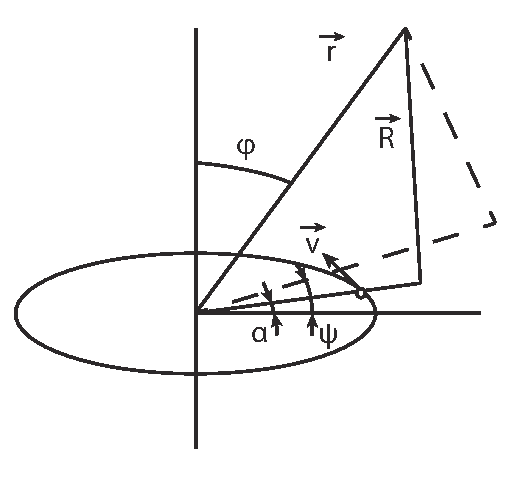
\includegraphics[width=\textwidth]{orbit}
\end{minipage}
\begin{minipage}{.5\textwidth}
    Для определения полей \( \vec{B} \) и \( \vec{E} \) необходимо найти
    \( \vec{A} \) и \( \phi \). Для начала найдем векторный потенциал
    движущегося заряда:
    \[
        \vec{A} = \frac{\mu_0}{4\pi}e\frac{\vec{v}_{t - \frac{R}{c}}}{R_{t - \frac{R}{c}}}.
    \]
    Положим \( R = r \). Введем сферическую систему координат \( (r,\ \theta,\ 
    \alpha) \). Тогда:
    \[
        \vec{A} = \frac{\mu_0}{4\pi}e\frac{\vec{v}_{t - \frac{r}{c}}}{r} =
        \frac{\mu_0}{4\pi}e\frac{a\omega\vec{e}_\alpha}{r},
    \]
\end{minipage}
где \( \vec{e}_\alpha \) -- взят в момент времени \( t - \cfrac{r}{c} \). Найдем
проекции \( \vec{A} \) на направления \( \vec{e}_r,\ \vec{e}_\phi,\ 
\vec{e}_\alpha \):
\[
    A_r = \vec{A}\cdot\vec{e}_n = \frac{\mu_0}{4\pi}\cdot\frac{e\omega a}{r}
    \cdot(-\sin\phi\cos\alpha\sin\psi + \sin\phi\sin\alpha\cos\psi) =
    \frac{\mu_0}{4\pi}\cdot\frac{e\omega a}{r}\sin\phi\sin(\alpha - \psi).
\]

Примем \( \psi = \omega t - \cfrac{\omega n}{c} \), тогда
\[
    A_r = \frac{\mu_0}{4\pi}\cdot\frac{e\omega a}{r}\sin\phi\sin\Omega,
\]
где \( \Omega = \cfrac{\omega r}{c} - \omega t + \alpha \).

Аналогично,
\[
    A_\phi = \frac{\mu_0}{4\pi}\cdot\frac{e\omega a}{r}\cos\phi\sin\Omega, \quad
    A_\alpha = \frac{\mu_0}{4\pi}\cdot\frac{e\omega a}{r}\cos\Omega.
\]
Теперь, зная проекции \( \vec{A} \), можем определить поле \( \vec{B} \):
\begin{gather*}
    \vec{B} = \rot\vec{A} = \frac{\mu_0}{4\pi}\cdot e\omega a\begin{vmatrix}
    \frac{\vec{e}_r}{r^2\sin\phi} & \frac{\vec{e}_\phi}{r\sin\phi} &
    \frac{\vec{e}_\alpha}{r} \\ \pder{}{r} & \pder{}{\phi} & \pder{}{\alpha} \\
    \frac{\sin\phi\sin\Omega}{r} & \cos\phi\sin\Omega & \sin\phi\cos\Omega
    \end{vmatrix} = \Biggl[\frac{\vec{e}_r}{r^2\sin\phi}(\cos\phi\cos\Omega - \\
    -\cos\phi\cos\Omega) + \frac{\vec{e}_\phi}{r\sin\phi}\left(\frac{\sin\phi}
    {r}\cos\Omega + \frac{\omega}{c}\sin\phi\sin\Omega\right) +
    \frac{\vec{e}_\alpha}{r}\biggl(\cos\phi\frac{\omega}{c}\cos\Omega - \\
    - \frac{\cos\phi}{r}\sin\Omega\biggr)\Biggr]\cdot\frac{\mu_0}{4\pi}\cdot e
    \omega a = \frac{\mu_0}{4\pi}\cdot e\omega a\cdot\Biggl[\vec{e}_\phi\left(
    \frac{\cos\Omega}{r^2} + \frac{\omega}{rc}\sin\Omega\right) + \\
    \vec{e}_\alpha\left(\frac{\omega}{rc}\cos\Omega - \frac{\sin\Omega}{r^2}
    \right)\cos\phi\Biggr].
\end{gather*}

В волновой зоне, пренебрегая \( \cfrac{1}{r^2} \), получим:
\[
    \vec{B} = \frac{\mu_0e\omega^2a}{4\pi rc}\left(\vec{e}_\phi\sin\Omega +
    \vec{e}_\alpha\cos\Omega\cos\phi\right).
\]

Считая в волновой зоне вблизи точки наблюдения волну плоской, получим:
\[
    \vec{E}=c\vec{B}\times\vec{e}_r = \frac{\mu_0e\omega^2a}{4\pi r}\left(
    \vec{e}_\phi\cos\phi\cos\Omega - \vec{e}_\alpha\sin\Omega\right).
\]
Так как в верхней полусфере \( \cos\phi > 0 \), то для излучения в ней имеет
место левая эллиптическая поляризация, переходящая при \( \phi = 0 \) в
круговую. Аналогично, в нижней полусфере имеет место правая поляризация в силу
\( \cos\phi < 0 \), переходящая в круговую при \( \phi = \pi \).

Для углового распределения интенсивности имеет место соотношение:
\( \ds \der{I}{\Theta} = r^2\cdot\mid{|\vec{P}|} \), где \( \vec{P} = \cfrac{1}
{\mu_0}\vec{E}\times\vec{B} \) -- вектор Пойнтинга. Определим его:
\[
    \vec{P} = \frac{1}{\mu_0}\cdot\frac{\mu_0^2e^2\omega^4a^2}{16\pi^2r^2c}
    \begin{vmatrix} \vec{e}_r & \vec{e}_\phi & \vec{e}_\alpha \\ 0 &
    \cos\phi\cos\Omega & -\sin\Omega \\ 0 & \sin\Omega & \cos\phi\cos\Omega
    \end{vmatrix} = \frac{\mu_0e^2\omega^4a^2}{16\pi^2r^2c}\vec{e}_r(\cos^2\phi
    \cos^2\Omega + \sin^2\Omega).
\]
Усредняя по времени, с учетом \( \mid{\cos^2\Omega} = \mid{\sin^2\Omega} = 1/2
\), имеем
\[
    \mid{|\vec{P}|} = \cfrac{\mu_0e^2\omega^4a^2}{32\pi^2r^2c}(1 + \cos^2\phi),
    \text{ откуда } \der{I}{\Theta} = \frac{\mu_0e^2\omega^4a^2}{32\pi^2c}
    (1 + \cos^2\phi).
\]
Теперь найдем полную интенсивность, учитывая, что в цилиндрически симметричном
случае \( d\Theta = 2\pi\sin\phi\d\phi \):
\[
    I = \frac{\mu_0e^2\omega^4a^2}{32\pi^2c}\int\limits_0^\pi (1 + \cos^2\phi)
    \cdot 2\pi\sin\phi\d\phi = \frac{\mu_0e^2\omega^4a^2}{6\pi c}.
\]

\vspace*{2em}
\emph{Ответ:}
\vspace*{-2.8em}
\begin{gather*}
    \mid{I} = \frac{\mu_0e^2\omega^4a^2}{6\pi c}, \quad \mid{\der{I}{\Theta}} =
    \frac{\mu_0e^2\omega^4a^2}{32\pi^2c}(1 + \cos^2\phi). \\
    \vec{B} = \frac{\mu_0e\omega^2a}{4\pi rc}\left(\vec{e}_\phi\sin\Omega +
    \vec{e}_\alpha\cos\Omega\cos\phi\right), \quad
    \vec{E} = \frac{\mu_0e\omega^2a}{4\pi r}\left(\vec{e}_\phi\cos\phi\cos\Omega
    - \vec{e}_\alpha\sin\Omega\right).
\end{gather*}

\newpage
%-------------------------------------------------------------------------------
\emph{761.} Заряд \( e \) движется с малой скоростью \( \vec{v} \) и ускорением
\( \vec{\dot{v}} \) в ограниченной области (задача \emph{760}). Определить
угловое распределение \( \der{I}{\Omega} \) и полное излучение \( I \).

\vspace*{2em}
\emph{Решение:}

Интенсивность излучения в направлении \( \vec{n} = \frac{\vec{r}}{r} \)
выражается через напряженность электрического поля \( \vec{E} \) в волновой
зоне:
\[
    \der{I}{\Omega} = \frac{c}{4\pi} E^2(t)R^2.
\]
Запишем выражение для электрического поля, воспользовавшись ответом предыдущей
задачи \emph{760}:
\[
    \vec{E} = \frac{e\vec{n}\times\left(\vec{n}\times\dot{\vec{v}}\right)}
    {c^2R}.
\]
Подставим его в первую формулу: 
\[
    \der{I}{\Omega} = \frac{e^2}{4\pi c^3} \left( \vec{n}\times \dot{\vec{v}}
    \right)^2,
\]
зная что \( d\Omega = 2\pi\sin\theta\d\theta \), найдем полное излучение:
\begin{gather*}
    dI = \frac{2\pi e^2}{4\pi c^3} \dot{v}^2 \sin^3\theta\d\theta; \\
    I = \frac{2\pi e^2}{4\pi c^3}\dot{v}^2\int\limits_0^\pi\sin^3\theta\d\theta
    = \frac{2e^2}{3c^3}\dot{v}^2.
\end{gather*}

\vspace*{2em}
\emph{Ответ:} \( I = \cfrac{2e^2}{3c^3}\dot{v}^2 \).
\end{document}
